\section{Training-Size Analysis}
\label{sec:capacity}

This exploratory analysis used three heads, three nested HBN training subsets,
and ten seeds, for 90 runs. Each selected checkpoint was evaluated on the same
75 MIPDB participants. The resulting 6,750 predictions are repeated evaluations
of those participants, not independent observations.

\subsection{Absolute performance and paired differences}
Table~\ref{tab:capacity-absolute} reports absolute correlations and parameter
counts. Table~\ref{tab:capacity-cells} gives candidate differences from the
size-matched baseline. The richer heads improved on all ten seeds in each cell.
Both 200-subject intervals and the MLP's 400-subject interval excluded zero;
the other intervals included zero.

\begin{table}[!htbp]
  \centering
  \small
  \caption{MIPDB correlations by HBN training size. SD is computed across ten
  seeds. The MLP has four hidden units.}
  \label{tab:capacity-absolute}
  \begin{tabular}{llrrr}
\toprule
Train $n$ & Head & Params & Mean Pearson & Seed SD \\
\midrule
200 & Mean-linear baseline & 513 & 0.527 & 0.011 \\
200 & Rich statistics & 2561 & 0.604 & 0.009 \\
200 & MLP (4 units) & 2569 & 0.582 & 0.025 \\
400 & Mean-linear baseline & 513 & 0.655 & 0.008 \\
400 & Rich statistics & 2561 & 0.711 & 0.008 \\
400 & MLP (4 units) & 2569 & 0.704 & 0.014 \\
800 & Mean-linear baseline & 513 & 0.645 & 0.008 \\
800 & Rich statistics & 2561 & 0.676 & 0.007 \\
800 & MLP (4 units) & 2569 & 0.662 & 0.012 \\
\bottomrule
\end{tabular}

\end{table}

\begin{table}[!htbp]
  \centering
  \small
  \caption{Paired candidate differences at each training size. W/T/L counts
  positive, zero, and negative seed differences. Intervals resample seeds and
  participants; p-values are exploratory.}
  \label{tab:capacity-cells}
  \begin{tabular}{rlrrrrr}
\toprule
Train $n$ & Head & Params & Mean $\Delta$ & 95\% CI & Holm $p$ & W/T/L \\
\midrule
200 & Rich statistics & 2561 & 0.078 & [0.019, 0.138] & 0.006 & 10/0/0 \\
400 & Rich statistics & 2561 & 0.056 & [-0.017, 0.139] & 0.006 & 10/0/0 \\
800 & Rich statistics & 2561 & 0.031 & [-0.048, 0.120] & 0.006 & 10/0/0 \\
200 & MLP (4 units) & 2569 & 0.056 & [0.019, 0.097] & 0.006 & 10/0/0 \\
400 & MLP (4 units) & 2569 & 0.049 & [0.006, 0.096] & 0.006 & 10/0/0 \\
800 & MLP (4 units) & 2569 & 0.017 & [-0.040, 0.076] & 0.006 & 10/0/0 \\
\bottomrule
\end{tabular}

\end{table}

\subsection{Changes in the candidate advantage}
Table~\ref{tab:capacity-contrasts} compares paired advantages between training
sizes. For example, 800 minus 200 subtracts the candidate's advantage at 200
subjects from its advantage at 800. All observed changes were negative. The
one-sided sign-flip tests retained the prespecified positive-change alternative,
which explains their large p-values; they are not tests for any change in
either direction. Only the MLP's 800-minus-400 bootstrap interval excluded zero.
The endpoint intervals included zero for both heads.

\begin{table}[!htbp]
  \centering
  \small
  \caption{Exploratory changes in the paired Pearson advantage. A negative
  value means a smaller candidate advantage at the larger training size.
  Holm p-values test the positive direction; SD describes seed differences.}
  \label{tab:capacity-contrasts}
  \begin{tabular}{llrrrr}
\toprule
Head & Contrast & Change in $\Delta$ & 95\% CI & Holm $p$ & SD \\
\midrule
Rich statistics & 800 minus 200 & -0.046 & [-0.112, 0.023] & 1.000 & 0.010 \\
Rich statistics & 400 minus 200 & -0.022 & [-0.069, 0.031] & 1.000 & 0.008 \\
Rich statistics & 800 minus 400 & -0.024 & [-0.065, 0.016] & 1.000 & 0.005 \\
MLP (4 units) & 800 minus 200 & -0.039 & [-0.090, 0.012] & 1.000 & 0.018 \\
MLP (4 units) & 400 minus 200 & -0.007 & [-0.044, 0.029] & 1.000 & 0.014 \\
MLP (4 units) & 800 minus 400 & -0.032 & [-0.061, -0.004] & 1.000 & 0.008 \\
\bottomrule
\end{tabular}

\end{table}

Table~\ref{tab:capacity-transfer} shows HBN validation and MIPDB correlations for
the selected candidate checkpoints. External scores did not select checkpoints.
Figure~\ref{fig:capacity-absolute} shows absolute performance, and
Figure~\ref{fig:capacity-seed-deltas} shows individual seed differences.
The joint intervals are shown once in Figure~\ref{fig:capacity-main}.

\begin{table}[!htbp]
  \centering
  \small
  \caption{HBN validation and MIPDB correlations for selected candidate heads,
  averaged over seeds.}
  \label{tab:capacity-transfer}
  \begin{tabular}{llrr}
\toprule
Train $n$ & Head & HBN validation $r$ & MIPDB $r$ \\
\midrule
200 & Rich statistics & 0.645 & 0.604 \\
400 & Rich statistics & 0.711 & 0.711 \\
800 & Rich statistics & 0.736 & 0.676 \\
200 & MLP (4 units) & 0.648 & 0.582 \\
400 & MLP (4 units) & 0.741 & 0.704 \\
800 & MLP (4 units) & 0.742 & 0.662 \\
\bottomrule
\end{tabular}

\end{table}

\begin{figure}[!htbp]
  \centering
  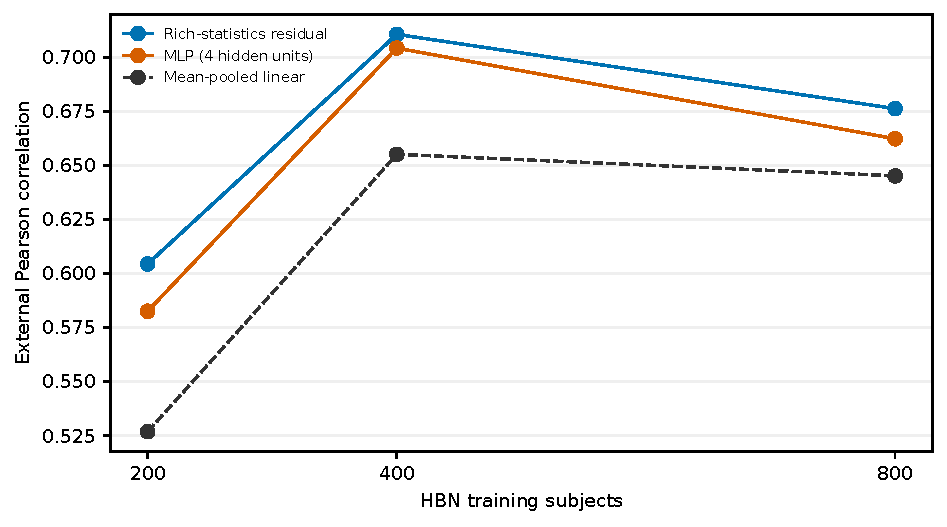
\includegraphics[width=0.80\linewidth]{presentation/capacity_data_regime_absolute.pdf}
  \caption{Absolute MIPDB correlations for each training size and head.}
  \label{fig:capacity-absolute}
\end{figure}

\begin{figure}[!htbp]
  \centering
  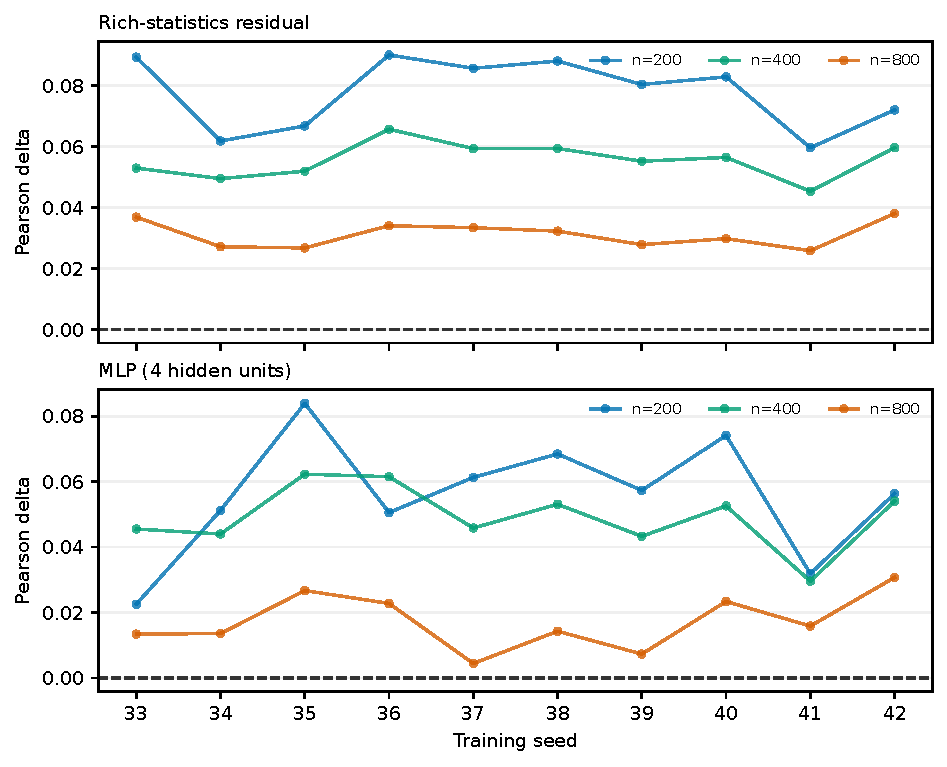
\includegraphics[width=0.80\linewidth]{presentation/capacity_data_regime_seed_deltas.pdf}
  \caption{Paired Pearson differences for the rich-statistics and four-unit
  MLP heads across seeds and HBN training sizes.}
  \label{fig:capacity-seed-deltas}
\end{figure}
